\subsection{Design Requirements}
The design requirements that are followed in this report are given by AIAA Request for Proposal \cite{RFP}, which are outlined in Table \ref{uno}.  Unlike many modern aircraft capable of seating 400+ passengers, the Toucan Sam Mark I has a maximum range of 3,500 nm, less than half of a Boeing 777-200, the seed aircraft for this project.  This is the biggest required design factor to consider while engineering this aircraft, as simply scaling a proven design is not realistic.  Furthermore, a design mission of 700 nm is referenced in the RFP, significantly altering the cruise portion of a design mission for this aircraft.  

\begin{table}[h!] 
    \centering
    \caption{RFP Requirements}
    \begin{tabular}{ |c||c| }\toprule
    \textbf{Category} & \textbf{Requirement} \\\hline\hline
    Capacity & 410 (10 crew, 400 passengers) \\\hline
    Payload & 94,000 lb (200lb per person, 30lb per occupant) \\\hline
    Range & 3,500 nm \\\hline
    Takeoff Field Length & 9,000 ft with a 35 ft obstacle \\\hline
    Landing Field Length & 9,000 ft \\\hline
    Approach Speed & 145 kts at end of design mission\\\hline
    Pressure & 8,000 ft pressure altitude at maximum flight altitude \\\hline
    Certification & Flying qualities should meet FAA 14 CFR Part 25.\\\hline 

    \end{tabular}\label{uno}
\end{table}
\clearpage
One self-imposed, yet extremely significant requirement Team Toucan placed on this aircraft is a fully composite wing and wing structure. While certainly not required, nor chosen out of necessity, this adaptation is driven by the desire to deliver maximum customer value over the decades of service seen by commercial aircraft.  Furthermore, it helps mitigate operations costs in the future, as fuel prices and their associated taxes continue to show a tendency to rise, especially in maturing markets.  Further quantitative discussion of the decision to utilize a hybrid design can be found in Section \ref{section: Structures and Loads}.

\subsection{Reference Mission Profile}
The mission profile consists of eight distinct subsections: taxi and takeoff, climb to a starting cruise altitude of 37,000 ft, cruise/step climb, descend, divert to an alternate airport 200 nm away, loiter for 30 minutes, descend, and land. This profile is illustrated below in Figure \ref{fig:missionprof}. 

\begin{figure}[!h]
    \centering
    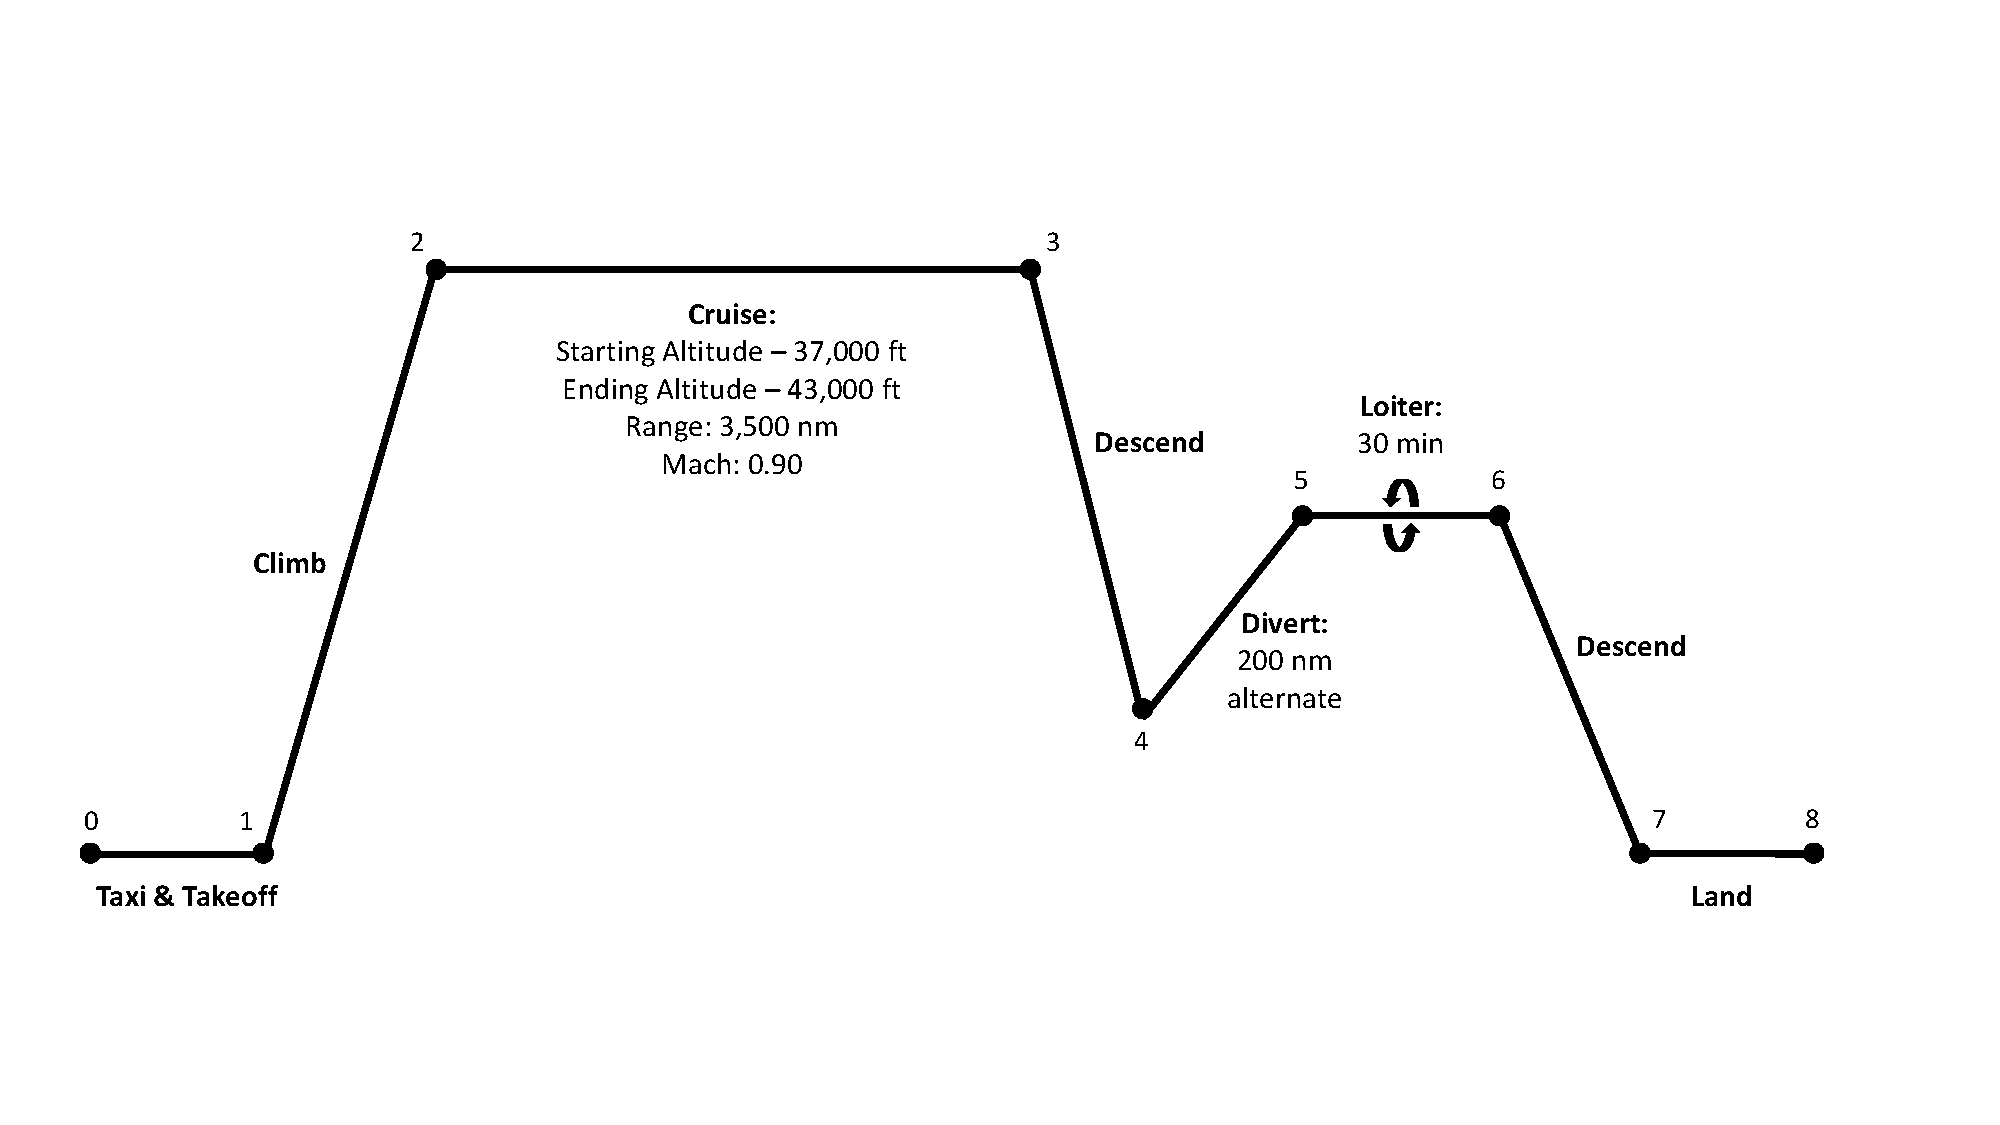
\includegraphics[width=1.0\textwidth]{Photos/Mission_Profile_(2-13-20).pdf}
    \caption{Typical Mission Profile}
    \label{fig:missionprof}
 \end{figure}

%\textcolor{red}{
%\begin{itemize}
    %\item AIAA: A description of the design missions defined for the proposed concepts for use in
%calculations of mission performance as per design objectives. This includes the
%selection of cruise altitude(s) and cruise speed/cruise Mach supported by pertinent
%trade analyses and discussion.
    %\item Discuss requirements (including those from the RFP and any additional derived requirements), constraints, and the design mission. \checkmark JJ
    %\begin{itemize}
        %\item Include a table of requirements.\checkmark JJ
        %\item \hl{Include a figure of the design mission with key mission segments labeled and details noted (e.g. cruise range and altitude).}
    %\end{itemize}
%\end{itemize}}